\documentclass[conf]{new-aiaa}
%\documentclass[journal]{new-aiaa} for journal papers
\usepackage[utf8]{inputenc}

\usepackage[utf8]{inputenc}

\usepackage{graphicx}
\usepackage{gensymb}
\usepackage{amsmath}
\usepackage[version=4]{mhchem}
\usepackage{siunitx}
\usepackage{subcaption}
\usepackage{longtable,tabularx}
\usepackage[export]{adjustbox}
\setlength\LTleft{0pt} 

\title{Direct Simulation of CMAS Infiltrating TBC Microstructure \\
\\
\textbf{EXTENDED ABSTRACT}}

\author{Brendon A. Cavainolo\footnote{Graduate Research Assistant, UCF Mechanical and Aerospace Engineering, AIAA Student Member.} and Michael P. Kinzel\footnote{Assistant Professor, UCF Mechanical and Aerospace Engineering, AIAA Senior Member.}}
\affil{University of Central Florida (UCF), Orlando, FL, 32816, United States}
\author{Ravisankar Naraparaju\footnote{High Temperature and Functional Coatings, DLR Institute of Materials Research}}
\affil{German Aerospace Center (DLR), Cologne, 51147. Germany}

\begin{document}

\maketitle
\section{Nomenclature}

{\renewcommand\arraystretch{1.0}
\noindent\begin{longtable*}{@{}l @{\quad=\quad} l@{}}
$APS$  & Air-Plasma Spray \\
$CFL$   & Courant-Friedrichs-Lewy Condition \\
$CMAS$  & Calcium-Magnesium-Alumino-Silicate \\
$EB-PVD$ &    Electron Beam Particle Physical Vapor Deposition \\
$GCI$ & Grid Convergence Index \\
$GRD$ & Giordano (CMAS viscosity model) \\
$HRIC$ & High-resolution Interface Capturing \\
$TBC$ & Thermal Barrier Coating \\
$VOF$ & Volume-of-Fluid \\
$\epsilon$ & ratio of results for a refinement level \\
$\theta$ & Contact angle \\
$\sigma$   & Surface Tension Coefficient \\
$\phi$ & Overall pore fraction of TBC \\
$\tau$ & Geometric Factor based on TBC \\
$\rho$ & density \\
$\mu s$ & microseconds
\end{longtable*}}

\section{Introduction}
\lettrine{T}{he} intake of Calcium-Magnesium-Alumino-Silicate (CMAS) particles by airplane engines poses a threat to the safety and durability of aircraft. For instance, in 1982, all four engines of a Boeing 747 on British Airways Flight 9 failed when the plane flew through a volcanic ash cloud made up of CMAS. When CMAS particles enter the engine, they melt due to the high temperatures and then solidify again on cooling lines \cite{Chen2015}. This can cause damage to compressor blades and thermal barrier coatings, leading to overheating and engine stall \cite{Chen2015}. Helicopters operating in sandy desert environments are at an even higher risk of CMAS damage \cite{Smialek}. The financial impact of CMAS ingestion can also be significant, as demonstrated by the closure of European airspace for six days following the eruption of Eyjafjallajökull in Iceland, which cost commercial airlines an estimated \$1.7 billion \cite{Thehumanconditionblog_2010}. It is crucial to understand how CMAS behaves inside aircraft engines to prevent damage to both airplanes and the global economy.

Thermal Barrier Coatings (TBCs) are ceramic layers applied to aircraft engine components, such as high-pressure turbine blades, to protect them from prolonged exposure to heat \cite{Bennett2005}. These coatings can reduce component temperatures from 1700 K to around 1200 K \cite{Sirigiri2018}. As higher temperature turbines are required for high thrust applications, it is essential to continue developing and understanding coatings that can more effectively reduce heat transfer in engines. TBC systems can be made using various materials and methods. One approach is to use EB-PVD 7YSZ-based coatings, which have better aerodynamic performance and strain compliance than APS TBCs in the top coat, the layer most susceptible to CMAS infiltration \cite{Renteria2007}. The columnar microstructure of an EB-PVD coating is shown in Fig. \ref{Fig1}, which shows both 'normal' and 'feathery' TBCs, and various stages between.

\begin{figure}[htp!]
\centering
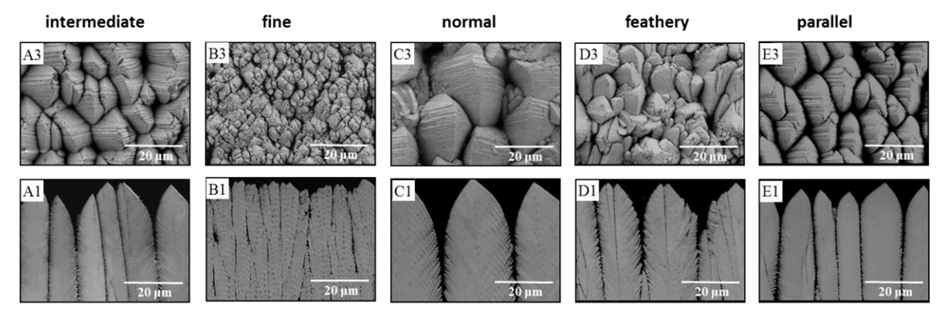
\includegraphics[width=.9\textwidth]{Figures/Fig1.png}
\caption{Various morphologies of EB-PVD TBCs under magnification \cite{Renteria2007}. The top panel depicts the TBC surface, while the lower panel shows a side view from a cut TBC. }
\label{Fig1}
\end{figure}

Melted CMAS infiltrates the inter-columnar gaps, and as the CMAS solidifies when the engine is not in use, the thermal expansion causes deformation in the TBC microstructure, which causes the desirable thermal insulation properties to degrade. The CMAS attack also causes a sintering phenomena to occur, which also erodes TBCs \cite{Peng2012}. As manufacturers seek to help aero-engines achieve higher temperatures for efficiency gains, molten CMAS is becoming more of a problem \cite{Boyce2012}. Depending on composition, most forms of CMAS melt between 1150 - 1250 \degree C \cite{Costa2019,Naraparaju2014,Wellman2010,Kramer2006}. The sintering occurs when the molten CMAS comes into contact with the TBC. In One such case, molten volcanic ash interacted with a YSZ TBC to form yttria iron garnet \cite{Xia2019}.

Current literature has explored several important aspects of CMAS interaction with aircraft engines. One such study includes a computational model exploring CMAS particle fan-blade interaction \cite{Vogel2018}. This study found a distribution of particle sizes that are likely to move past the fan stage in aeroengines \cite{Vogel2018}. Another important study investigated how the impact of CMAS particle size and chemical composition would affect the particle’s time to equilibrate on the nozzle guide vane. The particle’s properties were summarized using the thermal Stokes number. The ratio of particle impact temperature ($T_{p,imp}$) to the temperature of the fluid ($T_f$) was measured. The study showed that the temperature of particles with a $St_{th}$ below unity unity equilibrate with the temperature of the surrounding fluid in a fraction of the surrounding fluid’s response time. $St_{th}$ larger than unity led to particles that take much longer than the surrounding fluid’s response time to equilibrate with the surrounding fluid \cite{Bojdo2019}. This correlation was used as a validation methodology for this method \cite{Cavainolo2022}.
This work seeks to do the following: 1) Give an overview of necessary background information to understand the processes involved in simulating CMAS, 2) Provide details of a methodology in which CMAS infiltration into a TBC is directly resolved 3) Perform a design study on a parameterized TBC model to understand which dimensions lead to desirable infiltration properties, such as longer infiltration times, or less heat transfer to the TBC. Literature has proposed the use of analytical models to describe the infiltration of CMAS. In these models, the flow of CMAS is said to be analogous to open, and concentric pipe flow, with modifying factors based on properties of the TBC \cite{Naraparaju2017}. 

However, the flow could also be considered a capillary-driven flow. Here, models such as Waghmare and Mitra's \cite{WAGHMARE2010c, WAGHMARE2010117, WAGHMARE2010561} look at flow in a rectangular microchannel. Accounting for geometric differences, this model could serve as an analytical basis for CMAS infiltration in a TBC.

Shortcomings of this analytical model, including heat transfer analysis and thermal expansion processes, can be accounted for via simulation. 

This paper proposes the use of a finite-volume method (more specifically, the Eulerian Volume-of-Fluid Method), to resolve the infiltration of CMAS into an idealized TBC. Previous simulation-based infiltration models have used a FEM approach \cite{Sirigiri2018}, but this approach comes with several challenges, including difficulties with  resolving surface tension forces. Overall, the approach has the potential to push the understanding of infiltration processes. Previous work using this methodology has determined that experimental measurements for viscosity led to more accurate infiltration times. However, there was a large discrepancy between simulated and experimental infiltration times. This work seeks to further understand that discrepancy, and account for it in the simulation.

\section{Methodology}

The simulation methodology is explained in previous work \cite{Cavainolo2023, Cavainolo2022} and will be summarized here. The first step in simulating the infiltration of CMAS was to ensure the VOF method is a valid approach for capturing the melting-solidification of a CMAS particle. A mesh independence study was conducted in previous work \cite{Cavainolo2022}, and it is shown that melting particles between the solidus and liquidus temperatures of CMAS can be accurately resolved with the VOF method. For multiphase physics, the Eulerian Multiphase Volume-of-Fluid method was used to simulate the interactions between the two Eulerian phases, air, and CMAS.  Modeling surface tension properly is critical as the infiltration is driven mostly by capillary forces. The governing equations for the VOF method in Star-CCM+ ver. 18.02.008-R8 \cite{starccm} are shown in a finite-volume formulation and include the the Conservation of Mass,

\begin{equation}
\label{consMass:equation}
    \frac{\partial}{\partial t}\int_{V}\rho dV+\ \oint_{A}{v\bullet d\ A}=\ \int_{V}\left(S\right)dV\ ,\ S=\ \sum_{i}{S_{a_i}\rho_i}
\end{equation}

\noindent,the Conservation of Momentum,

\begin{equation}
\label{consMomentum:equation}
    \frac{\partial}{\partial t}\int_{V}\rho vdV+\oint_{A}{\rho v\times v}\bullet\ dA=\oint_{A}{\rho I\bullet d\ A}+\oint_{A}{T\bullet d\ A}+\int_{V}\rho gdV+\ \int_{V}{f_bdV}-\sum_{i}\int_{A}{a_i\rho_iv_{d,i}\times v_{d,i}dA}
\end{equation}

\noindent and the Conservation of Energy,

\begin{equation}
\label{consEnergy:equation}
   \frac{\partial}{\partial t}\int_{V}\rho EdV+\oint_{A}\left[\rho Hv+p+a_i\rho_i{H_iv}_{d,i}\right]\bullet dA=-\oint_{A}{{\dot{q}}^{\prime\prime}\bullet d A}+\oint_{A}{T\bullet v d A}+\int_{V}{S_EdV}+\ \int_{V}{f_bdV}.
\end{equation}

\noindent Equations 3-5 couple to the Eulerian Multiphase VOF Transport Equation which is formulated as follows 

\begin{equation}
\label{VOFtrans:equation}
    \frac{\partial}{\partial t}\int_{V}{a_idV}+\ \oint_{A}{a_i\mathbit{v}\bullet d\ A}=\ \int_{V}{\left(S_{a_i}-\frac{a_i}{\rho_i}\frac{D\rho_i}{Dt}\right)dV-\int_{V}{\frac{1}{\rho_i}\mathrm{\nabla}\bullet}}\left(a_i\rho_iv_{d,i}\right)dV
\end{equation}

\noindent In these equations, the subscript i denotes a particular phase (in this case, air or CMAS), $a_i = V_i/V$ is the volume fraction of a particular phase, and $S_a_i$ is a source term defined by the initialization of the phases. The VOF method implements a technique called High-Resolution Interface Capturing (HRIC). HRIC imposes a Courant number limit (i.e. Co = 1.0), and if the Courant number is exceeded, then the HRIC scheme reverts back to a standard upwind scheme, which results in a smeared interface. This smeared interface can be corrected by implementing temporal subcycling. The general idea of temporal subcycling is shown in Equation \ref{eq:GeneralTempSubCycle}, where the right-hand side of the equation is a single source term that combines the right-hand side contributions from Equation \ref{VOFtrans:equation}. 

\begin{equation}
\label{eq:GeneralTempSubCycle}
    \alpha^{n+\Delta t}V - \alpha^{n}V + \int_{t^{n}}^{t^{n+\Delta t}}( \ \sum_{A}\alpha_{f}(s) v \cdot da) = \int_{t^{n}}^{t^{n+\Delta t}}(S(\alpha (s),...)ds
\end{equation}

\noindent In this work, an implicit multi-stepping version of this temporal subcycling is employed, which gives an unconditionally stable solution, and a sharp interface is achieved if $\frac{CFL}{N_{imp}} \leqslant 0.5 $. The sub-iterations calculated with Equation \ref{eq:implicitMultiStep1} are summed up to get the overall contribution for the whole time step.

\begin{equation}
\label{eq:implicitMultiStep1}
    \alpha_{i+1}V - \alpha_{i}V + \tau( \ \sum_{A}\alpha_{f,i+1}(\tau) v \cdot da) = \tau(S(\alpha^{n+\Delta t},...) ~for~ i = 1, 2, ..., N
\end{equation}

A drawback of using the VOF method for the infiltration is the very small time steps required to resolve the CMAS infiltration. So, adaptive time-stepping combined with sub-iterations was used to balance computational speed and accuracy. A free-surface condition was enforced so that the Courant number ($Co = \frac{u \Delta t}{\Delta x}$) at the interface was around 1.0. Such a criterion is often demanded to limit the interfacial motion to only a cell. The VOF method requires the use of a segregated solver (i.e. the energy equation is solved in a separate system of equations). This solver is second-order accurate in space, and first-order accurate in time. However, the lower-order time accuracy is offset by the implicit multi-stepping in the segregated VOF solver, described in Equations \ref{eq:GeneralTempSubCycle} - \ref{eq:implicitMultiStep1}. 

The preliminary model was  set up as a 2D geometry, a depiction of which is shown in Fig. \ref{Fig3}. Where the feathery pattern shown on the left is repeated downward until the TBC column is 200 $\mu m$ deep. This is half the size of a typical TBC column. The mesh is an unstructured trimmer mesh. The effect of contact angle was captured using prism layers at the wall. Boundary conditions, and domain dimensions, are summarized in Fig. \ref{dimensions} and Table \ref{tab:boundaryConditions}. The top of the domain is a velocity inlet, and the bottom of the domain was set as a pressure outlet with a pressure smaller than the reference pressure. This pressure difference between the inlet and outlet was set up so that a pressure gradient pushes the CMAS particle downward. The sides of the domain are also set as pressure outlets. Conjugate heat transfer was considered by setting the TBC as a solid region, the walls of the TBC were prescribed a temperature gradient of 1 $K/\mu m$, such that the top of the coating is close to a typical operating temperature for an engine environment. The gradient is defined this way because a typical YSZ EB-PVD TBC is around 400 $\mu m$ deep, and manages to be around 400 K cooler at the bottom of the TBC than the top, such that the operating temperature is below the melting point of the materials used. It should be noted there is only a gradient in the x-direction, so any walls on the same x-plane will have a constant temperature, and any walls along the same y-plane will have a temperature that varies.

The air phase was modeled as a constant-density fluid in this simulation. Thus, it is necessary to account for air getting trapped within the feather gaps as it would prevent the CMAS from infiltrating those gaps. To accomplish this, the interface between the fluid and solid regions was set as a porous boundary, only allowing air to escape. The rate at which air was allowed to escape was based on a user-defined external pressure, inertial resistance, and viscous resistance, which were 0 Pa (reference), 100 (dimensionless), and 1 m/s respectively. Hence, the air can escape the fluid domain at a maximum velocity of 0.01 m/s according to Eq. \ref{porous:equation} \cite{starccm}.

\begin{equation}
\label{porous:equation}
    \Delta P = -\rho (\alpha |v_n| + \beta)v_n
\end{equation}

\begin{figure}[htp!]
\centering
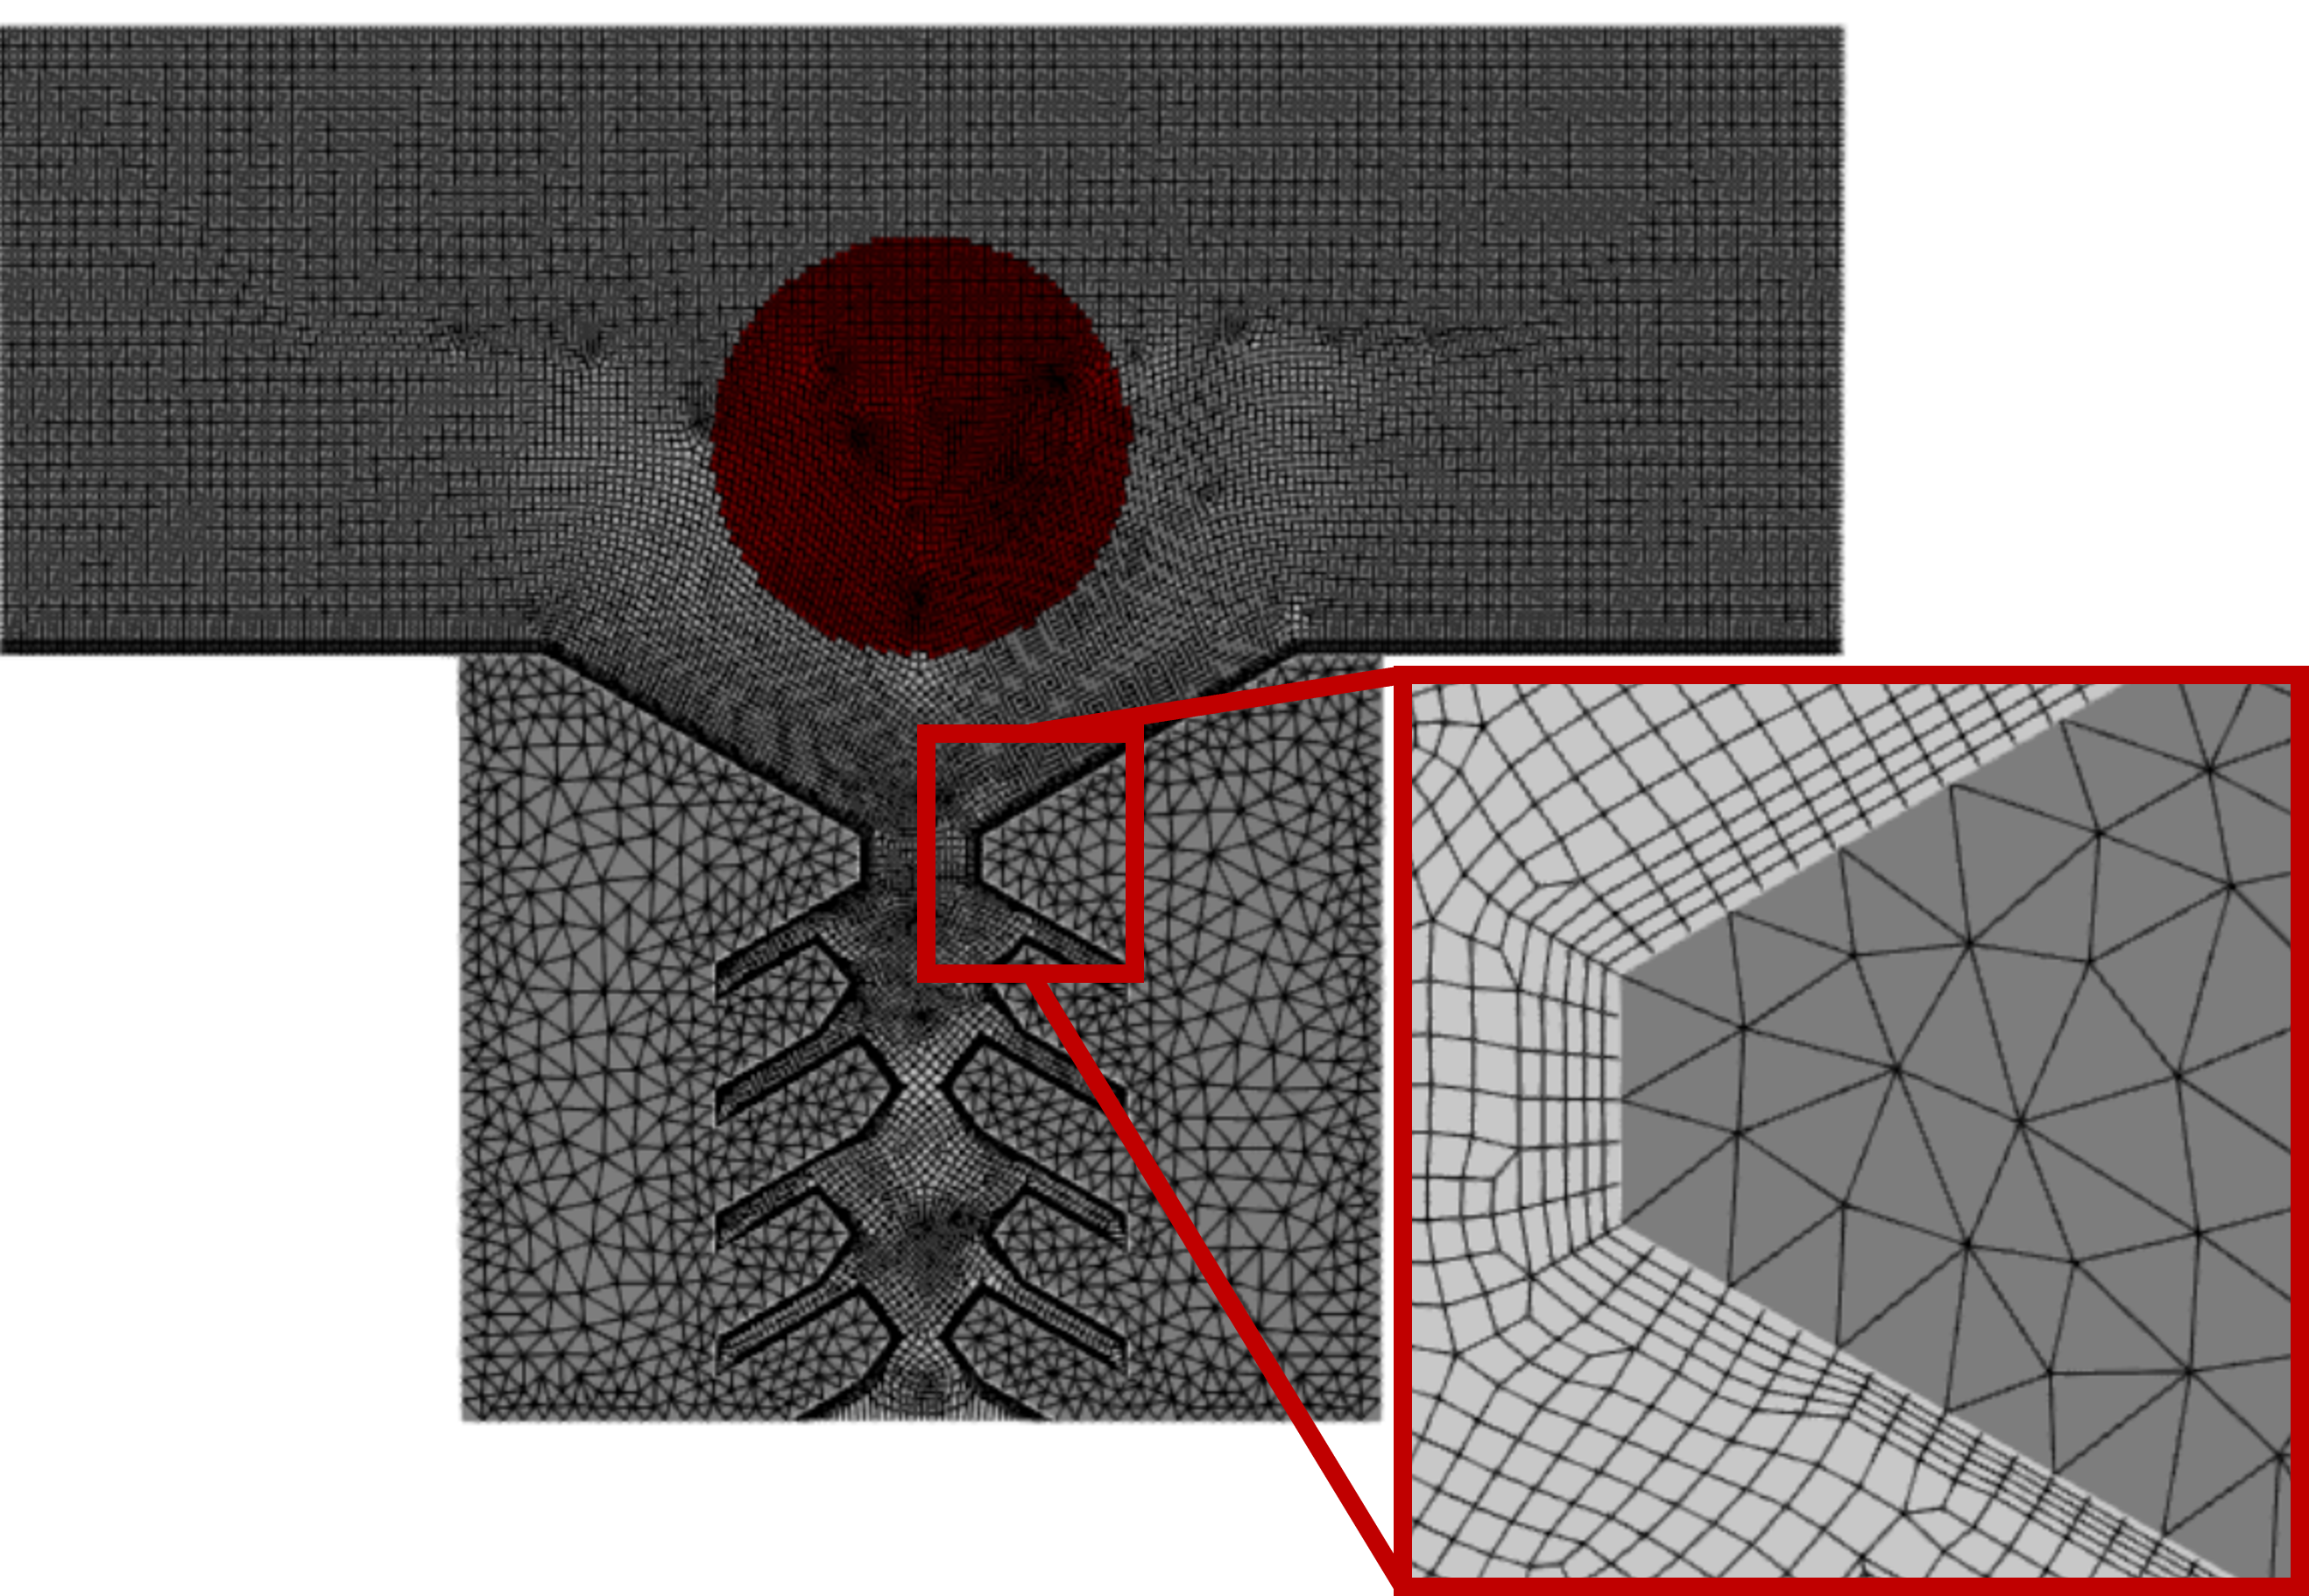
\includegraphics[width=.75\textwidth]{Figures/Fig3.png}
\caption{Zoomed out mesh, and  mesh zoomed in around wall region}
\label{Fig3}
\end{figure}

\begin{figure}[htp!]
\centering
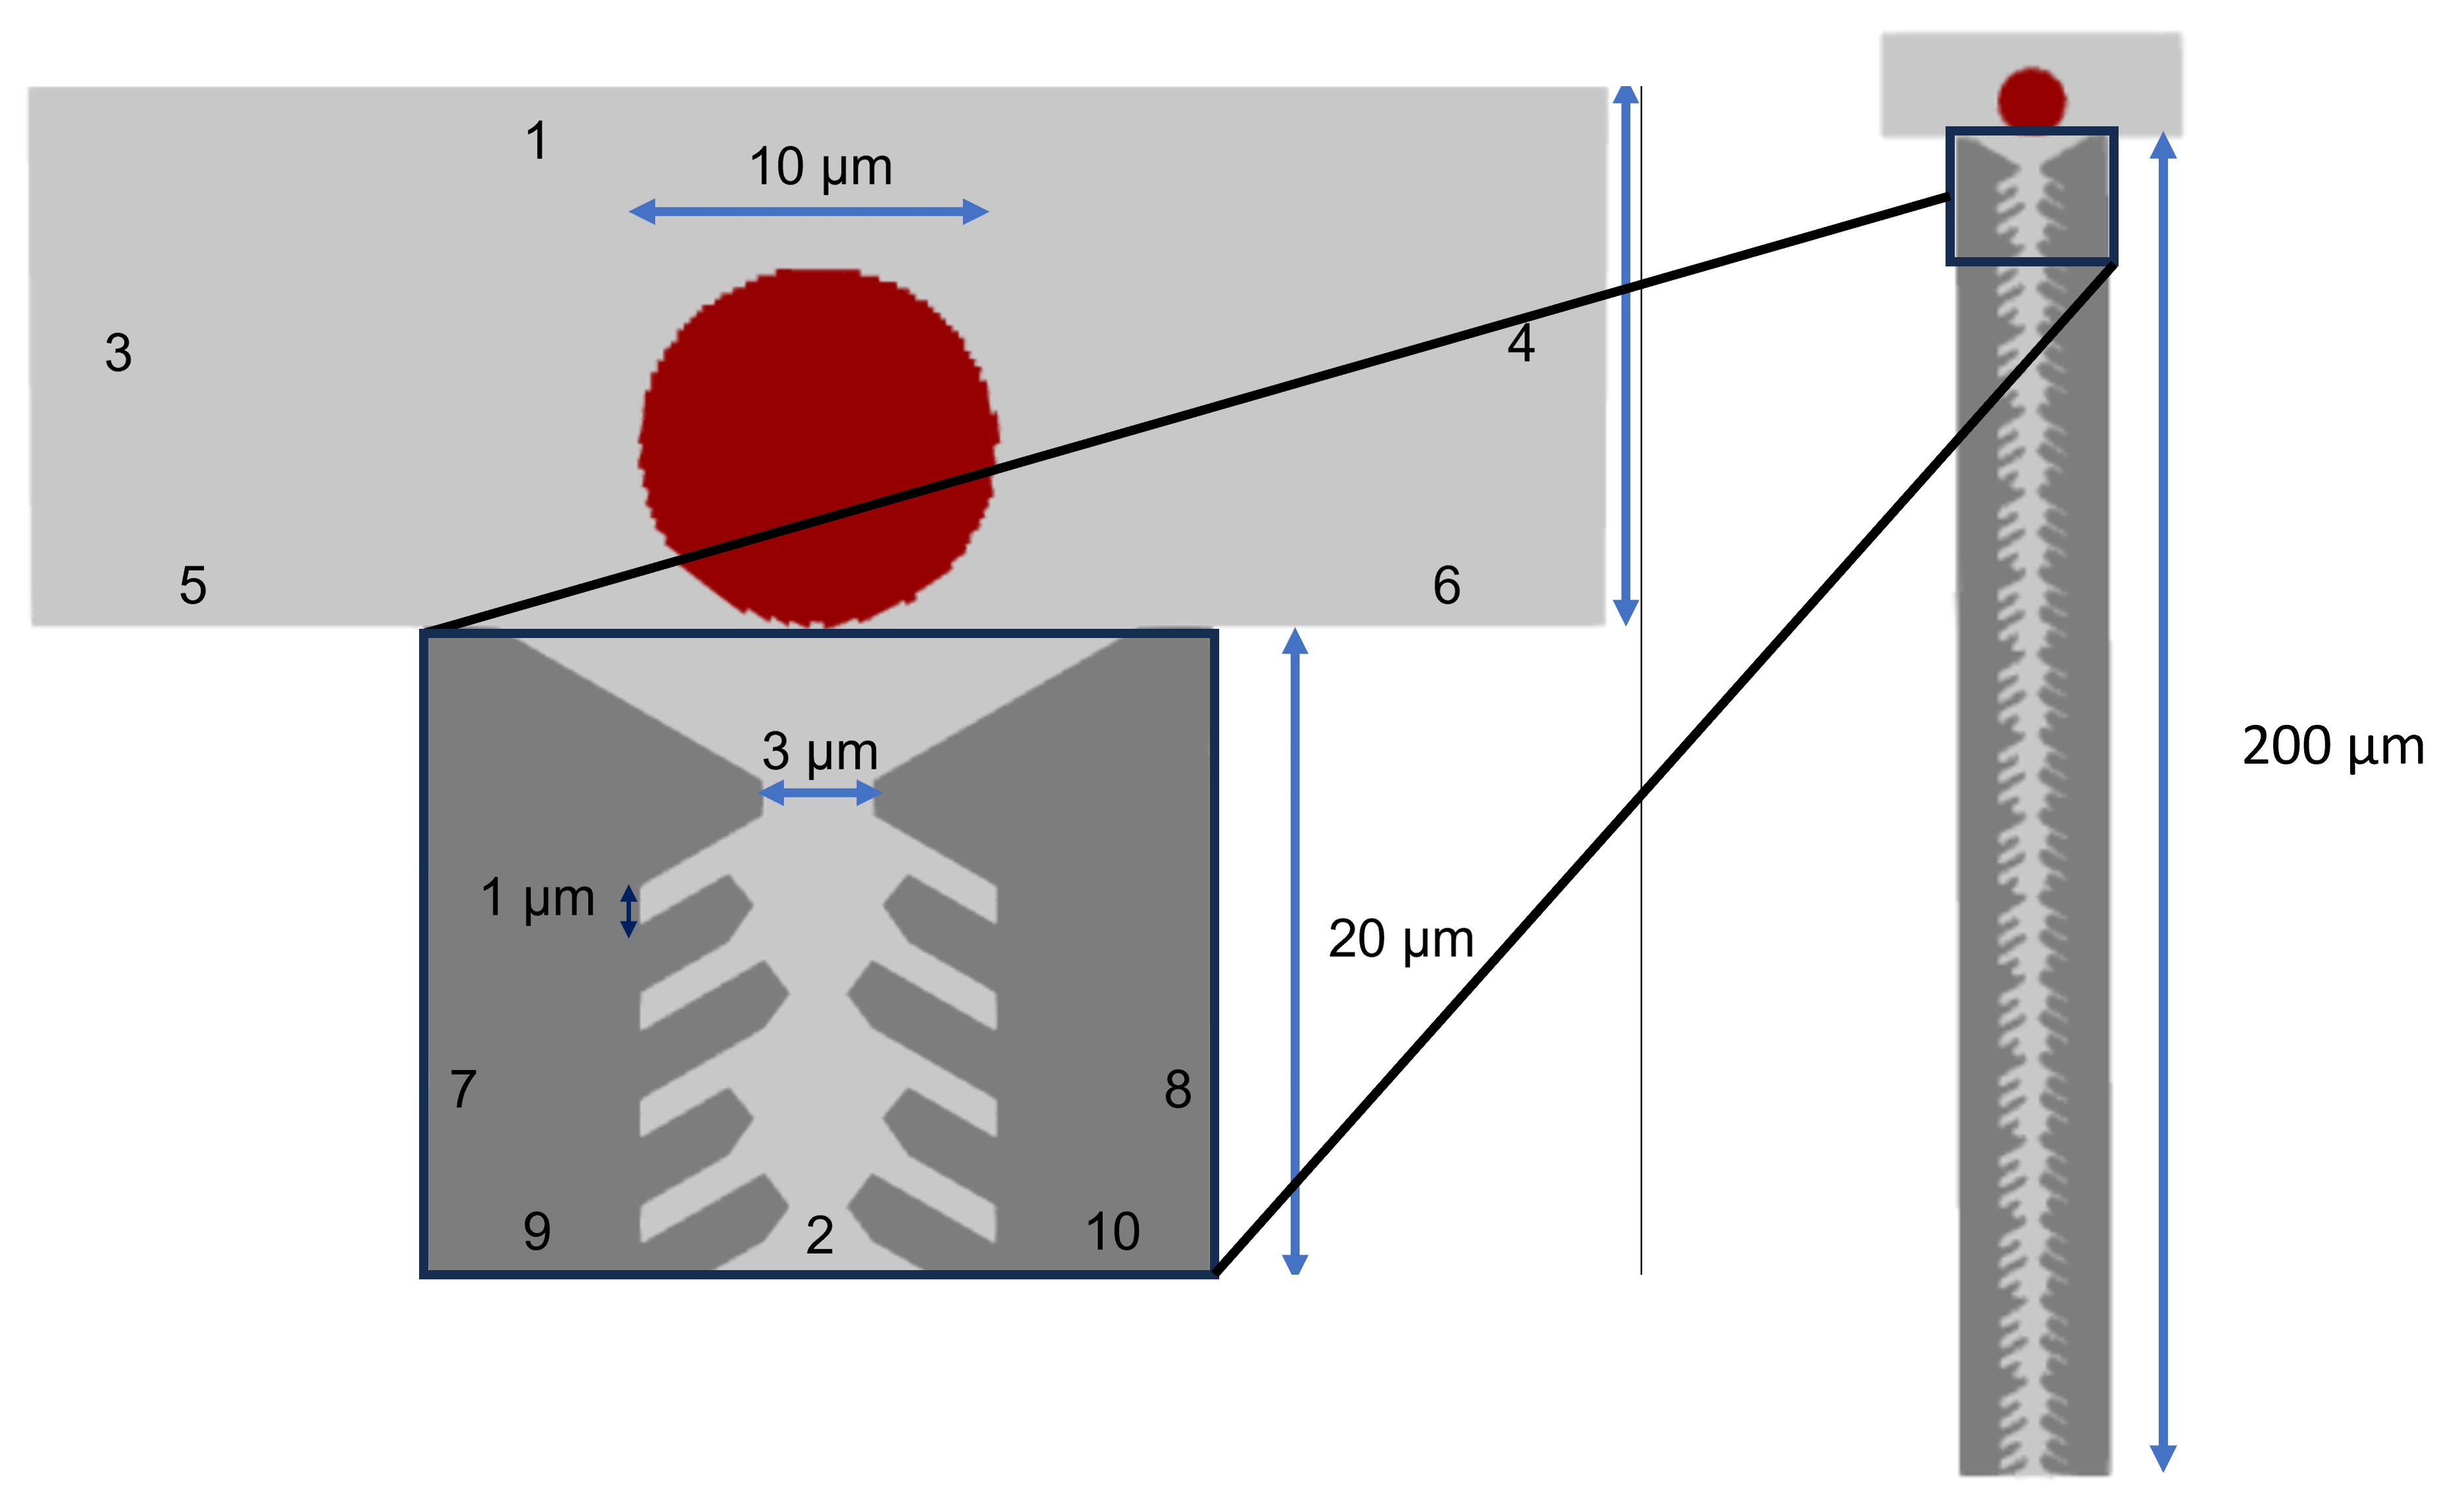
\includegraphics[width=.75\textwidth]{Figures/dimensions.png}
\caption{Geometry with labeled dimensions and boundary conditions}
\label{dimensions}
\end{figure}

\begin{table}
\caption{\label{tab:boundaryConditions} Summary of Labaled Boundary Conditions (Pressure values with respect to reference pressure)}
\centering
\begin{tabular}{lcccccc}
\hline
Label & Boundary Condition& Value (Units)\\\hline
1& Velocity & 0.1 $\mu m/s$\\
-& $\frac{\partial T}{\partial x}$& 1 $K/\mu$ m\\
2& Pressure& -25000 Pa\\
-& $\frac{\partial T}{\partial x}$& 1 $K/\mu$ m\\
3-4& Pressure& 10000 Pa\\
-& $\frac{\partial T}{\partial x}$& 1 $K/\mu$ m\\
5-10& $\frac{\partial T}{\partial x}$& 1 $K/\mu$ m\\
\hline
\end{tabular}
\end{table}


The 2D geometry and mesh can be seen in Fig \ref{Fig3}. The preliminary results presented here will use this 2D formulation. The wall contact angle of the CMAS phase is expected to be somewhere between 40 and 60 degrees based on experiments \cite{Naraparaju2019}. These values are temperature dependent though. For simplicity, a constant wall contact angle of 40 degrees was chosen.  


The thermal gradient described above for boundary conditions was also used as the initial condition for both the fluid region and solid region, except for the CMAS particle, which had a variable starting temperature. The fluid domain's initial velocity was set such that there was a very small downward velocity. This is done because it helps with convergence in the first calculations in the simulation. The CMAS particle was set at 0.2 m/s downward to ensure a quick interaction with the TBC. The reference pressure is 1 atm. While it could potentially make more sense to use engine operating pressures for the simulation's reference pressure, this domain was set up to be more in line with experiments conducted by Naraparaju et al. \cite{Naraparaju2014, Naraparaju2017, Naraparaju2019} to ensure the comparison to experimental data is as accurate as possible. Gravity was also enabled to capture any infiltration effects from buoyancy. Turning on gravity also adds the Boussinesq Approximation to the energy equation to account for natural convection. However, the effects of natural convection are low due to the small domain size.

Properties of both the CMAS and the TBC can affect the infiltration. Some of these properties are widely documented, such as thermal conductivity of the TBC \cite{Han2023}. Table \ref{tab:CMAS and TBC properties} shows the properties for both the CMAS and the TBC used in these simulations. Blank entries are properties not required by the models selected (in this case, for the solid TBC region).


\begin{table}
\caption{\label{tab:CMAS and TBC properties} Summary of thermal and physical properties of CMAS and TBC}
\centering
\begin{tabular}{lcccccc}
\hline
Property & CMAS& TBC\\\hline
Thermal Conductivity (W/m-K)& 1.15 \cite{Bakal2017} & tabular \cite{Han2023} \\
Specific Heat (J/kg-K)& 900 \cite{KAKUDA2015350} & tabular \cite{Han2023} \\
Density (kg/m$^3$)& 2690 \cite{BANSAL20153901}& 4800 \cite{KAKUDA20092583}\\
Dynamic Viscosity (Pa-s)& Polynomials w.r.t Temperature \cite{Sirigiri2018}& -\\
Latent Heat of Fusion (J/kg)& $1.973x10^7$ \cite{Costa2019}& -\\
Surface Tension (N/m)& 0.4 \cite{Bravo2020}& -\\
\hline
\end{tabular}
\end{table}

One important departure from previous work, however, is the use of the melting-solidification flow stop model to achieve a more accurate infiltration time. It is proposed that varying the flowability threshold for the solid CMAS can bring the solution more in line with the experimental infiltration results. 

\section{Preliminary Results}

\subsection{Mesh Sensitivity Study}
Mesh sensitivity was conducted based on the infiltration depth at 0.1 s of physical time. This parameter was chosen because it is a parameter for which experimental data exists, and is therefore important for validation in this study. The physical time to extract the infiltration depth was chosen because beyond that time, error accumulates in the simulation, causing the mass of CMAS to grow beyond the initial value, causing the result to be non-physical. This non-physical phenomenon can be seen in the coarsest mesh in Figure \ref{fig:mesh-a}, and the result becomes more clear in Figure \ref{fig:mesh-b} - \ref{fig:mesh-d}. The results in Figure \ref{fig:meshSensResults} and Table \ref{tab:meshSensResults} show asymptotic convergence. With such incredibly small variations with coarser mesh sizes, a mesh with a base size of ${1.4x10^{-7}}$ m will be used for further simulations. Performing the formal grid convergence index (GCI) calculations \cite{ECA2014104, celik2008procedure} shows that the results in Table \ref{tab:meshSensResults} mean this is monotonically converging, because  $0<\epsilon_{21}/\epsilon_{32}=\ 0.004<1$, and a GCI of $7.5x10^{-4}$.

\begin{figure}[htp!]
    \begin{subfigure}{0.5\textwidth}
        \centering
        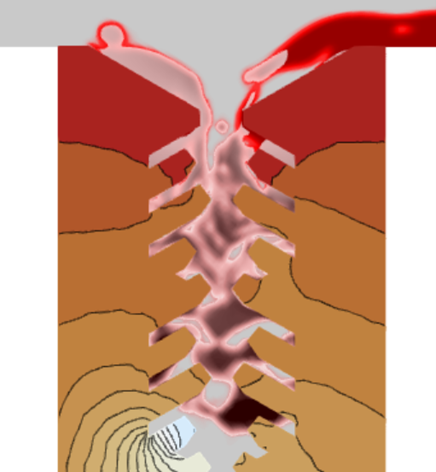
\includegraphics[scale=0.75]{Figures/coarsestMesh.png}
        \caption{$2.1x10^{-7}$}
        \label{fig:mesh-a}
    \end{subfigure}
    \begin{subfigure}{0.5\textwidth}
        \centering
        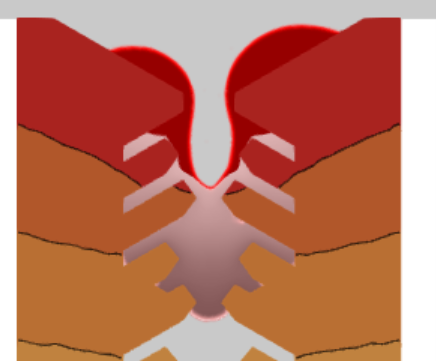
\includegraphics[scale=0.75]{Figures/fineMesh.png}
        \caption{$1.4x10^{-7}$}
        \label{fig:mesh-b}
    \end{subfigure}
    \begin{subfigure}{0.5\textwidth}
        \centering
        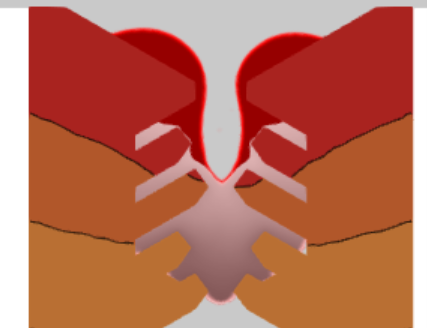
\includegraphics[scale=0.75]{Figures/finerMesh.png}
        \caption{$1.0x10^{-7}$}
        \label{fig:mesh-c}
    \end{subfigure}
    \begin{subfigure}{0.5\textwidth}
        \centering
        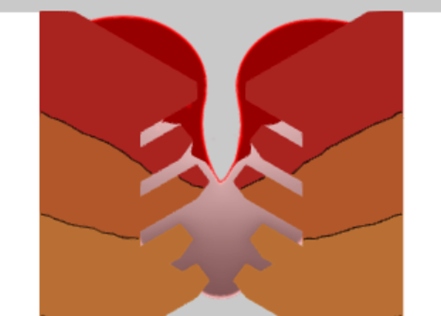
\includegraphics[scale=0.75]{Figures/finestMesh.png}
        \caption{$7.5x10^{-8}$}
        \label{fig:mesh-d}
    \end{subfigure}
    \caption{CMAS Infiltration at different levels of mesh refinement}
    \label{fig:mesh-refine}
\end{figure}

\begin{figure}
    \centering
    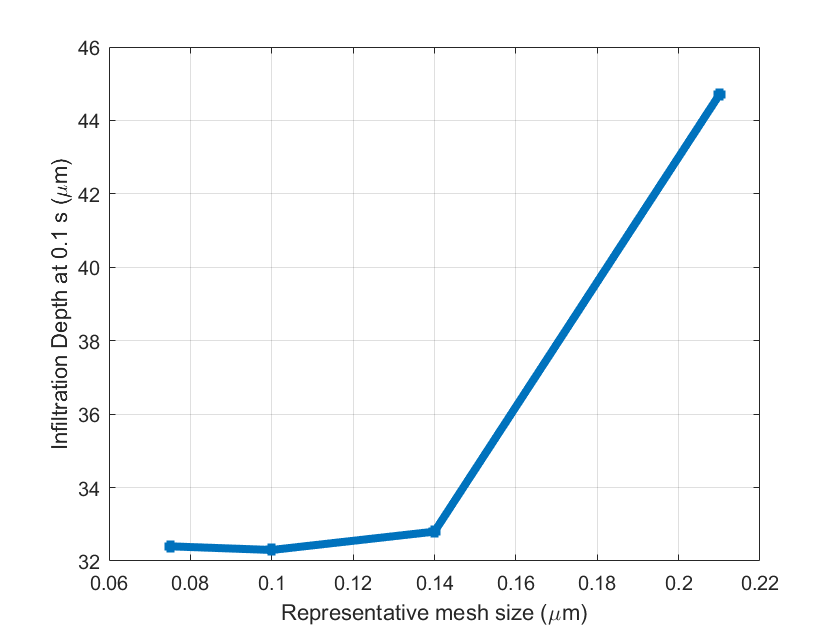
\includegraphics[scale=0.55]{Figures/infilDepthMesh.png}
    \caption{Infiltration Depth (m) as a function of representative mesh size (m}
    \label{fig:meshSensResults}
\end{figure}

\begin{table}[]
    \centering
    \caption{Table with Mesh Sensitivity Results from Figure \ref{fig:meshSensResults}}
    \begin{tabular}{c|c}
       Representative Mesh Size (m)  & Infiltration depth at 0.1 s (m) \\
       \hline
        2.1x10-7 & 4.465663e-05 \\
        1.4x10-7 & 3.280286e-05 \\
        1.0x10-7 & 3.233177e-05 \\
        7.5x10-8 & 3.238081e-05
    \end{tabular}
    \label{tab:meshSensResults}
\end{table}

\subsection{Analytical Benchmark}
Experimental results in Figure \ref{fig:RaviInfilDepth} for infiltration depth v. time are compared to simulations. These experimental results come from the German Aerospace Center, and the material used for “CMAS 1” is consistent with the material defined in the simulation. Unfortunately, the data is much farther advanced in time and with much less time resolution than the simulation. Numerical errors in mass conservation in the simulation tend to add up to a point where the result is non-physical around 0.5 s, making it difficult to compare to any time points in Figure \ref{fig:RaviInfilDepth}.  So instead, the simulation data will be compared to the open-pipe and concentric pipe models described in Naraparaju et. al. \cite{Naraparaju2019}. The formulations for this model can be seen below. 

\begin{figure}
    \centering
    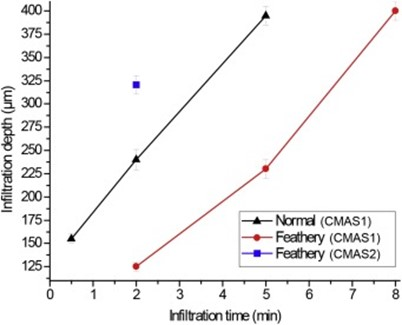
\includegraphics{Figures/RaviInfilDepth.jpg}
    \caption{Experimental Infiltration Depth v. Time Measurements}
    \label{fig:RaviInfilDepth}
\end{figure}

\begin{equation}
    t=\frac{\mu r\ h^2}{2\sigma k cos\theta}
\end{equation}

\noindent here, t is the infiltration time, r is the radius open for infiltration, h is the infiltration depth, $\mu$,$ \sigma$, $\theta$ are viscosity, surface tension, and contact angle respectively \cite{Naraparaju2017,ZHAO201474}. The parameter k represents the porosity and varies depending on whether the open-pipe or concentric-pipe model is being used. Some difficulties arise here, as some of the properties in the above equation vary nonlinearly with temperature, so initial values will be used for the calculations. The open-pipe model defines k as the following

\begin{equation}
    k_o=\frac{r^2\phi^2}{8\tau\left(1-\phi\right)^2}
\end{equation}

\noindent here $\phi$ is the overall pore fraction, and $\tau$ is a geometric factor based on a ratio of area of the column to area of the feather arms, and it was found to be 2.31 for feathery microstructures \cite{Naraparaju2019}.The concentric pipe model is similar, but defines k as

\begin{equation}
    k_o=\frac{\phi}{8\tau^2}b^2\left[1+\frac{a^2}{b^2}+\left(1-\frac{a^2}{b^2}\right)\frac{1}{ln\left(a/b\right)}\right]
\end{equation}

\noindent where a and b are the outer radii of the concentric pipes \cite{Naraparaju2019}. The results of the benchmark to the analytical models are shown in Figure \ref{fig:analytBench}. While the simulation under-predicts depth compared to the models, it is important to note that these are of the same order of magnitude, which supports the idea of neglecting chemical interactions in future simulations, as they may not be first-order contributors to the infiltration process.

\begin{figure}[h!]
    \centering
    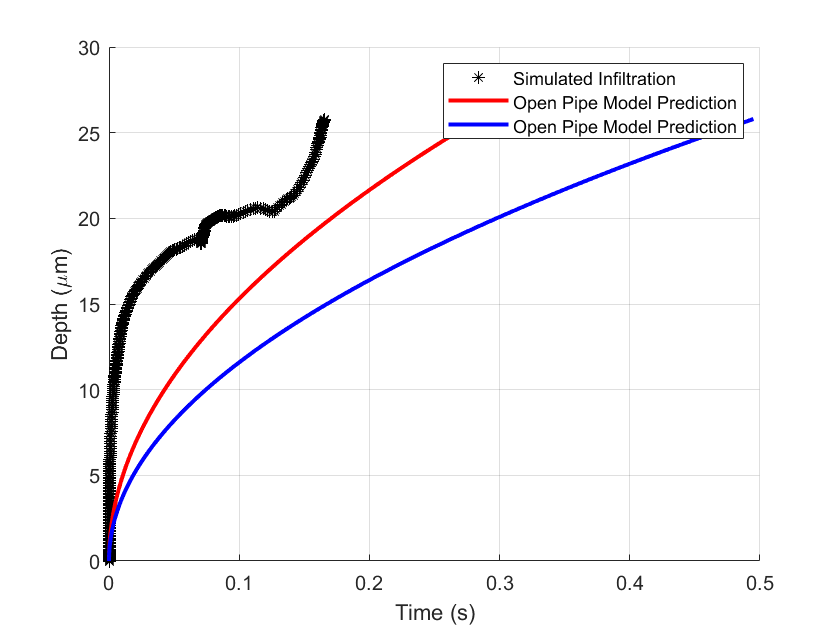
\includegraphics[width=0.75\textwidth]{Figures/analyticalBenchmark.png}
    \caption{Comparison of Simulation Results to Analytical Models for infiltration depth}
    \label{fig:analytBench}
\end{figure}


\subsection{Characterization Based on Viscosity}
In this study, two different formulations of the CMAS dynamic viscosity were evaluated: the GRD viscosity model \cite{Giordano2008}, and experimental viscosity measurements \cite{Naraparaju2019}.  The difference between the experimental and GRD viscosity is shown in Fig. \ref{viscosity}, where the experimental viscosity is higher throughout the entire temperature range. Simulations were run with both the experimental and GRD viscosity, using a temperature-based polynomial to approximate the data. Figure \ref{infilTimeVisc} shows that the infiltration time for the experimental viscosity is around 2.5x slower as the GRD viscosity. However, the infiltration times measured here are several orders of magnitude faster than those measured in experiments \cite{Naraparaju2019} if the infiltration rate curves are extrapolated out to the experimental TBC depth \cite{Stein2023}. 

Computational results from other work show a larger difference between the experimental and numerical infiltration times \cite{Sirigiri2018}. However, those results treated both the experimental and GRD viscosity as constant values of 6, and 0.6 Pa-s respectively. Those results also did not account for conjugate heat transfer effects or the existence of air in the domain (i.e. no surface tension effects). So it makes sense that the results presented here would show overall longer infiltration times. The results presented in this section also do not account for any melting-solidification processes and have the same starting temperature such that the particle is fully-liquid throughout the simulation. An image of how the viscosity varies with temperature throughout the domain is shown in Fig. \ref{fig:TempAndVisc}.

\begin{figure}[htp!]
\centering
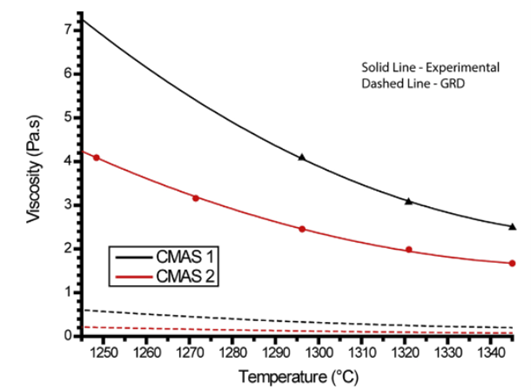
\includegraphics[width=.5\textwidth]{Figures/viscosity.png}
\caption{Experimental v. GRD Viscosity Curves}
\label{viscosity}
\end{figure}


\begin{figure}[htp!]
\centering
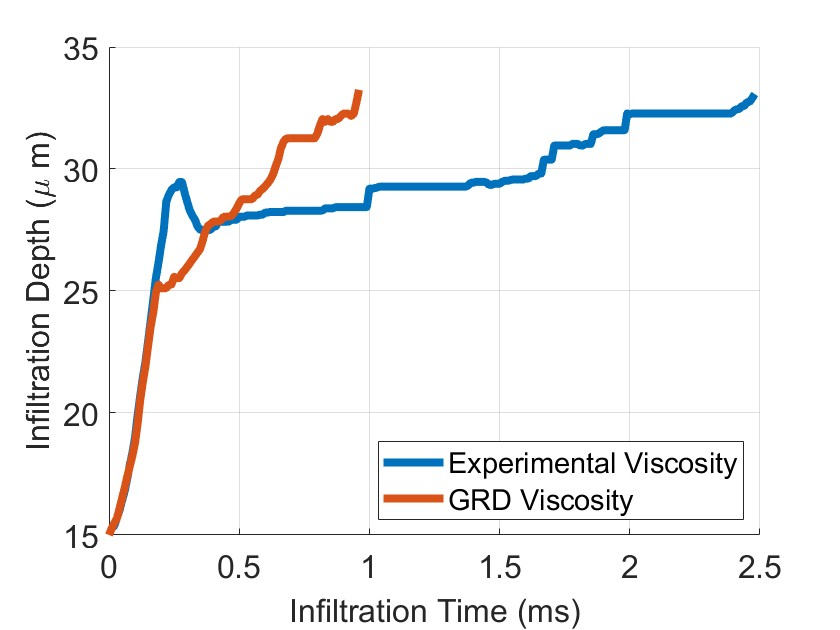
\includegraphics[width=.5\textwidth]{Figures/viscosity_v_time_curves.jpg}
\caption{Experimental v. GRD Infiltration Time}
\label{infilTimeVisc}
\end{figure}

\begin{figure}[!htb]
\centering
\begin{subfigure}{0.4\textwidth}
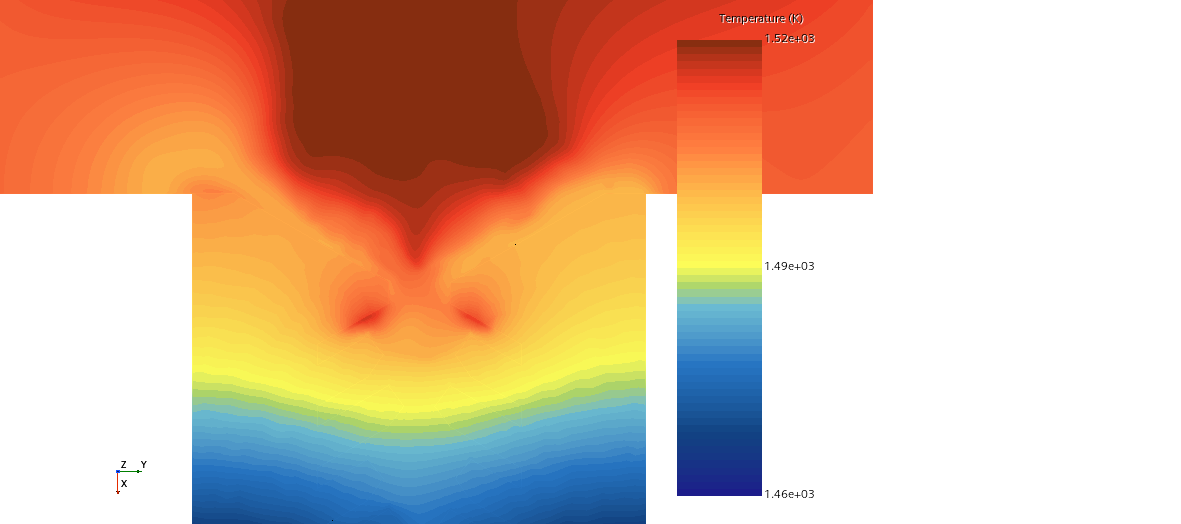
\includegraphics[scale=0.2]{Figures/TemperatureView_image_00270.png} 
\caption{Temperature at Final Time Step}
\label{fig:Temper}
\end{subfigure}
\begin{subfigure}{0.4\textwidth}
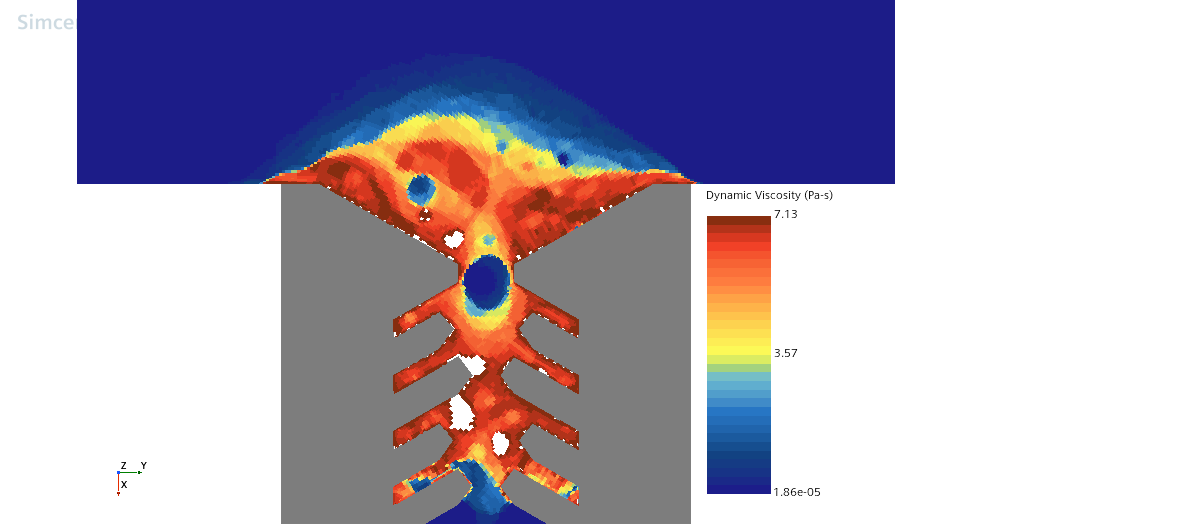
\includegraphics[scale=0.2]{Figures/Viscosity_View_image_00270.png}
\caption{Viscosity at Final Time Step}
\label{fig:viscVary}
\end{subfigure}

\caption{Viscosity Variation with Temperature in Domain}
\label{fig:TempAndVisc}
\end{figure}

\subsection{Expected Results}
Results from Naraparju et. al. \cite{Naraparaju2019} show that the concentric pipe model has a shorter infiltration depth than their experimental results at a given time, and the open pipe model has a farther infiltration depth than the experiments. This information is summarized in \ref{tab:compareInfilDepth}. If the simulation data from \ref{fig:analytBench} is cleaned up and extrapolated with a base-10 logarithmic curve fit, a depth can be estimated for the simulation at the same time as the experiment. However, this result shows a much shorter infiltration depth than both analytical models and the experiment. IOt is expected trhat this result will change once the simulation is refined to handle longer runtimes. The result will also be refined my finding a more robust extrapolation method.

\begin{table}[htb!]
    \centering
    \caption{Comparison of infiltration depth ($\mu m$) at 120 s of infiltration time for experiments and analytical models}
    \begin{tabular}{c|c}
        Result & Depth at 120 s ($\mu m$) \\
        \hline
        Experimental Measurement & 125 \\ Concentric Pipe Model & 95 \\ Open Pipe Model & 176\\
        Extrapolated Simulation & 38
    \end{tabular}

    \label{tab:compareInfilDepth}
\end{table}



\clearpage
\bibliography{sample}

\end{document}
